\chapter{Related Works}
\label{chapter:related}

%\minitoc
\chapterwithfigures{\nameref*{chapter:related}}
\chapterwithtables{\nameref*{chapter:related}}

\ifthenelse{\boolean{skipRelated}}{\endinput}{}

\section{Deep Learning for Computer Vision}

\ac{CNN} have been for a long-time the \textit{defacto} method for \acs{NN} for \ac{CV}
\citep{fukushima1980neocognitron,lecun1999lenet}. In 2012, with larger datasets and better hardware
(\ie \acs{GPU}), \cite{krizhevsky2012alexnet} imposed \ac{DL} models as the best performing
algorithms for images. In the 2010's decade, multiple major improvements were made but the one of
the latest best performing models \citep{tan2019efficientnet} is mainly based on two architectural changes:
residual connections allowing training of very deep networks \citep{he2016resnet} and normalization
of intermediate activations \citep{ioffe2015batchnorm}. Another major factor of recent \ac{CNN}
improvements is better training procedure \citep{wightman2019resnetstrikesback}, which includes
optimizer \citep{kingma2014adam}, learning rate scheduling, strong data augmentations
\citep{muller2021trivialaugment,hingyi2018mixup,zhong2017erasing}, and regularizations
\citep{gal2016dropout,gao2016stochasticdepth}.

More recently, the Transformer architecture \citep{vaswani2017transformer}, originally designed for
machine translation in \ac{NLP}, was applied to images. Using an encoder structure similar to BERT
\citep{devlin2018bert}, ViT \citep{dosovitskiy2020vit} considered patches of pixels as tokens.

\section{Continual Learning}

Usually, when training a \ac{CNN}, we assume the dataset is immutable and \textit{i.i.d.}: no new
image nor new classes will be learned. The knowledge acquired on one dataset A can be
\textit{transferred} to another dataset B with different classes using \textbf{transfer learning}
\citep{razavian2014transferlearning}. However, in that case, the new model, while being efficient on
the dataset B, cannot classify the classes of dataset A.

\textbf{Continual Learning} aims to learn a continually changing dataset without forgetting the
previous knowledge. \eg a model could learn at first to classify among 10 classes, then add 10 more
classes, \etc. Continually learning an increasing number of classes is easily doable if the data of
previous classes is accessible. However, it may not always be the case: privacy reasons are often
raised ---think medical data or federated learning's user data. In that situation, learning new
classes lead to a \textbf{catastrophic forgetting} \citep{robins1995catastrophicforgetting} of
previous classes.

What is continual, iid, forgetting

evaluation, multi-head, single-head

class incremental, domain incremental, new class and new domain incremental. \cite{lomonaco2017core50}


\section{Rehearsal}

\begin{figure}[tb]
    \begin{center}
        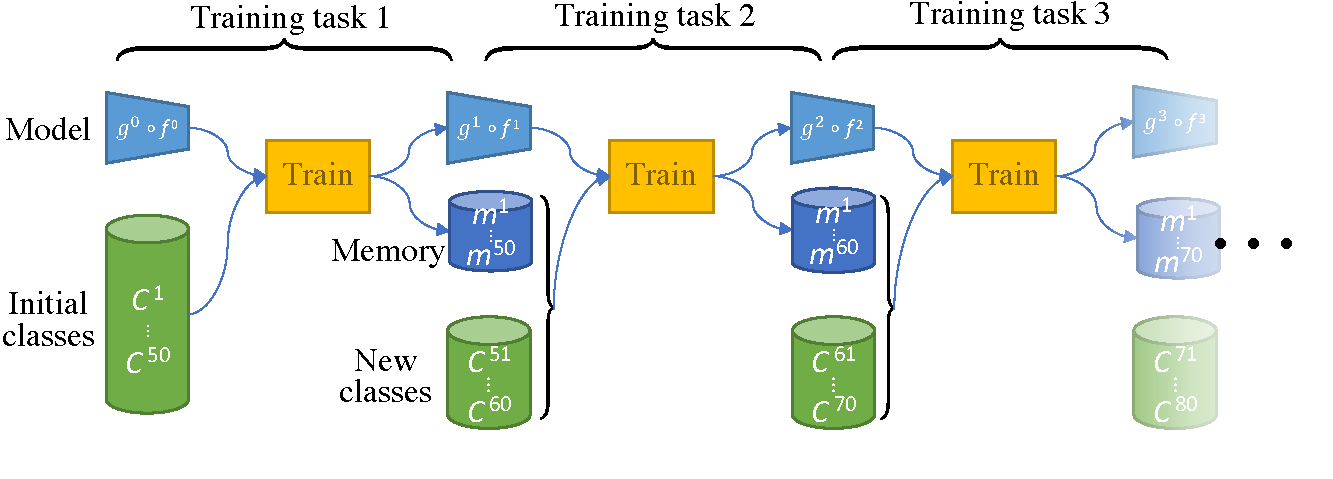
\includegraphics[width=0.8\linewidth]{images/podnet/protocol}
    \end{center}
    \caption{\textbf{Training protocol for incremental learning}. At each training task we learn a
        new set of classes, and the model must retain knowledge about \textit{all} classes. The
        model is allowed a \textit{limited} memory of samples of old classes.}
    \label{fig:related_protocol}
\end{figure}

\autoref{fig:related_protocol}


\section{Regularization-based Approaches}

\begin{figure}[tb]
    \begin{center}
        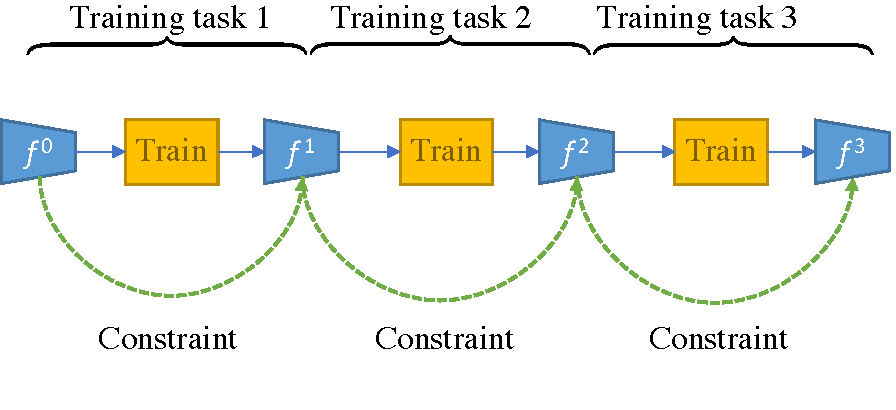
\includegraphics[width=0.8\linewidth]{images/related/continual_regularizations.pdf}
    \end{center}
    \caption{\textbf{Training protocol for incremental learning}. At each training task we learn a
        new set of classes, and the model must retain knowledge about \textit{all} classes. The
        model is allowed a \textit{limited} memory of samples of old classes.}
    \label{fig:related_regul}
\end{figure}

\subsection{Weight-based}

\citep{lesort2019regulshortcomings} showed that


\subsection{Gradient-Based}

\subsection{Output-based}

\section{Dynamic Strategies}



\section{Optimization}

